\documentclass[12pt,a4paper]{article}
\usepackage{url}
\usepackage[backend=bibtex]{biblatex}
\usepackage{caption}
\usepackage[utf8]{inputenc}
\usepackage{enumerate}
\usepackage{tabularx}
\usepackage{graphicx}
\usepackage{float}
\usepackage{color}
\usepackage{amssymb,amsmath,wasysym}

\addbibresource{bib1.bib}

\begin{document}

\title{Computational Intelligence, SS2017, Assigment 2}

\author{%
\name{Lucas Reeh}
\email{lreeh@student.tugraz.at}
}
\date{\today}

\begin{titlepage}
   \begin{center}
     \begin{huge}
		   %% Update assignment number here
           \textbf{Assignment 2}
     \end{huge}
   \end{center}

   \begin{center}
     \begin{large}
           Computational Intelligence, SS2017
     \end{large}
   \end{center}

   \begin{center}
 \begin{tabularx}{\textwidth}{|>{\hsize=.33\hsize}X|>{\hsize=.33\hsize}X|>{\hsize=.33\hsize}X|} 

           \hline
           \multicolumn{3}{|c|}{\textbf{Team Members}} \\
           \hline
           Last name & First name & Matriculation Number \\
           \hline
           Reeh & Lucas & 00630128 \\
           \hline

     \end{tabularx}
   \end{center}
\end{titlepage}

\tableofcontents
\listoffigures

\newpage

\section{Regression with Neural Networks}

\subsection{Simple Regression with Neural Networks}

\begin{enumerate}[a)]
  
%%%%%%%%%%%%%%%%%%%%%%%%%% 1.1 a)
  
  \item \textbf{Learned function}
  
Following plots show the learned function after ``fitting'' data sets to neural
network Python scikit-learn\autocite{scikit} using different numbers of neurons
in 1 hidden layer in den netowrk.
  
\begin{figure}[H]
	\centering
  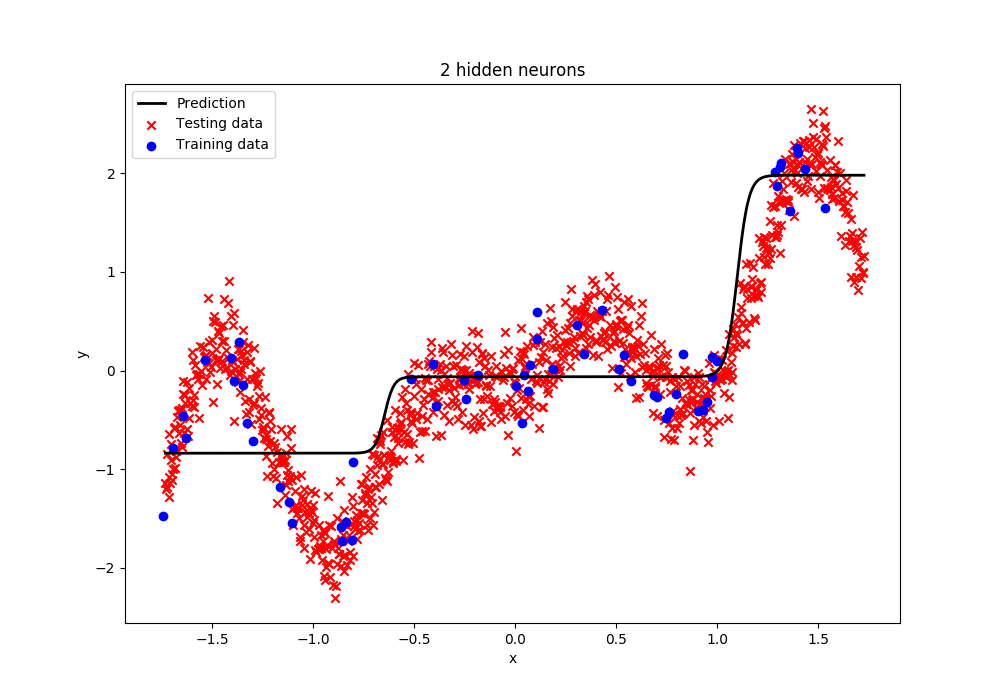
\includegraphics[width=0.9\textwidth]{figures/1_1_a_hn_2.png}
	\caption{NN Learned function $h_n=2$}
	\label{1_1_a_hn_2}
\end{figure}

\begin{figure}[H]
	\centering
  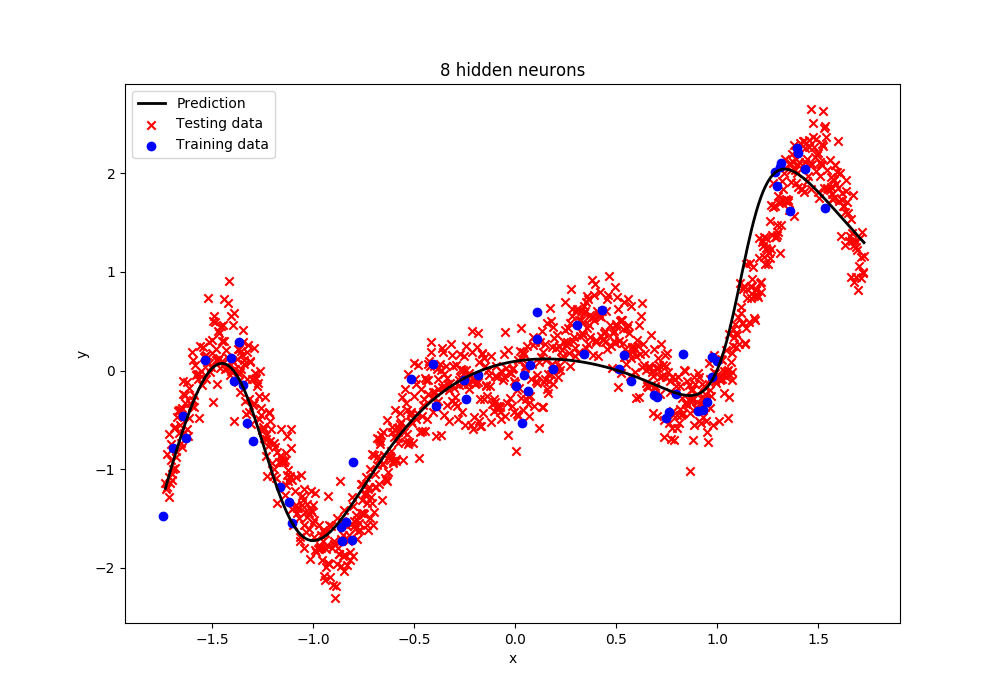
\includegraphics[width=0.9\textwidth]{figures/1_1_a_hn_8.png}
	\caption{NN Learned function $h_n=8$}
	\label{1_1_a_hn_8}
\end{figure}

\begin{figure}[H]
	\centering
  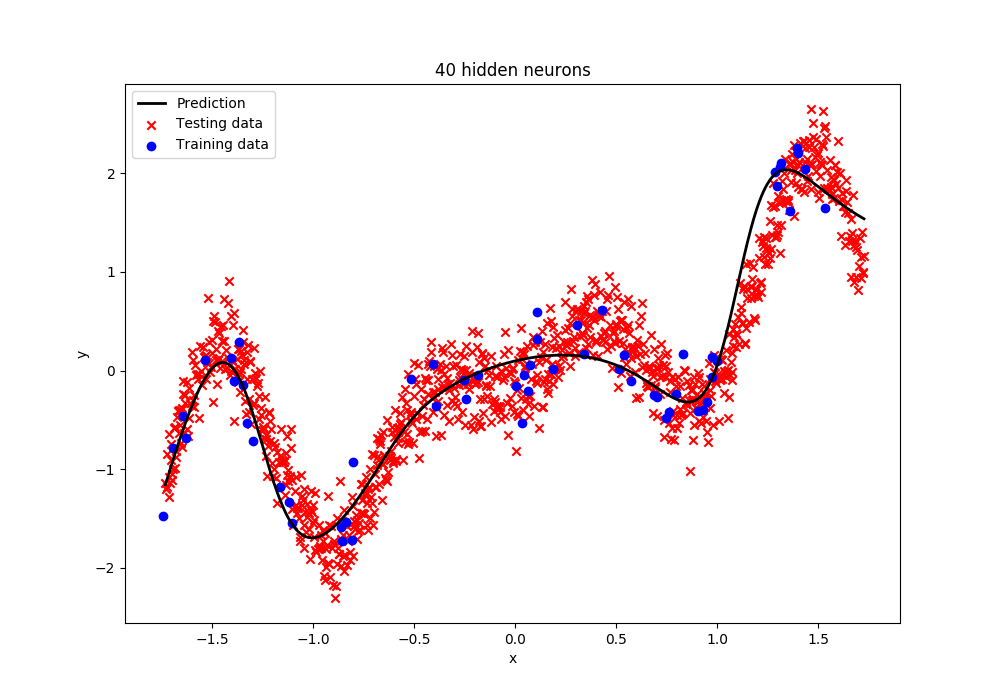
\includegraphics[width=0.9\textwidth]{figures/1_1_a_hn_40.png}
	\caption{NN Learned function $h_n=40$}
	\label{1_1_a_hn_40}
\end{figure}
  
\textbf{Discussion}

$2$ ``neurons'' in the hidden layer are cleary an underfitting parametrization
(missing a lot of data points), $h_n = 8$ seems to miss data points where $ x =
0.0$, $40$ nodes tend to overfit a little (see slope around $x = 1.5$ is going
up again). As shown in Figure \ref{1_1_a_hn_100} $100$ hidden layers seem to
recognize the concarve slope around $x = 0.0$ but is also overfitting at $x >
1.2$. From this Traning data there is no saying if this curve should be added. I
added it just because it is possible.

\begin{figure}[H]
	\centering
  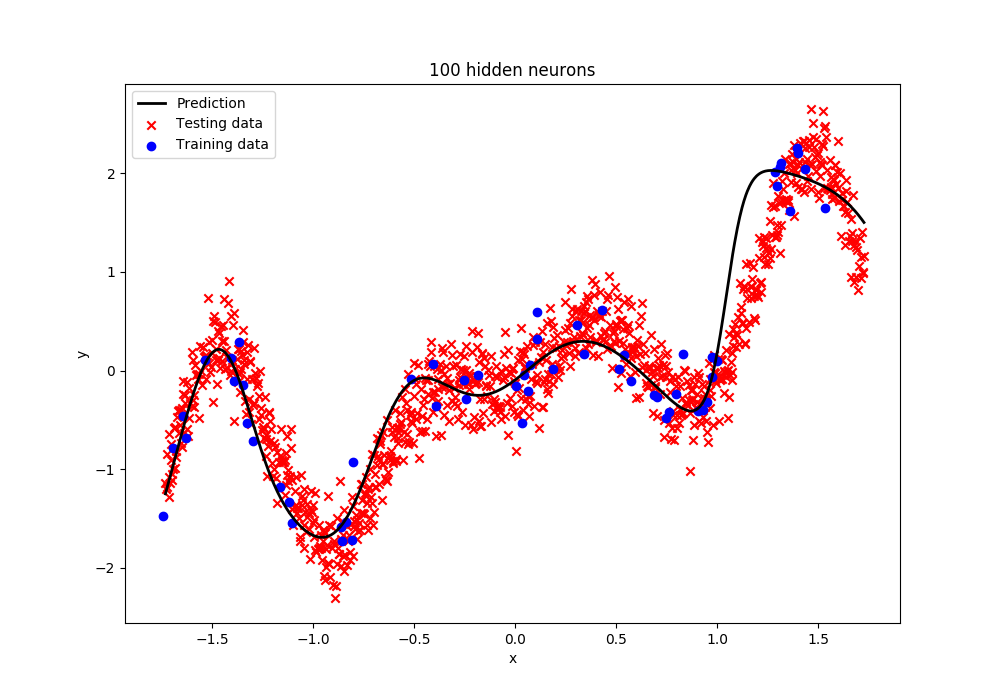
\includegraphics[width=\textwidth]{figures/1_1_a_hn_100.png}
	\caption{NN Learned function $h_n=100$}
	\label{1_1_a_hn_100}
\end{figure}

%%%%%%%%%%%%%%%%%%%%%%%%%% 1.1 b)

  \item \textbf{Variability of the performance of deep neural networks}

\texttt{seed\_state} = $1..9$:

\textbf{Results, Discussion}

\begin{itemize}
  \item minimum, maximum, mean and standard deviation

\texttt{Training MSE \\
- min = 0.040917789313120616 \\
- max = 0.05225074774663281 \\
- mean = 0.0449607719274836 \\
- std = 0.003249135660634265 \\
\\
Test MSE \\
- min = 0.09765403812014457 \\
- max = 0.23390967685837927 \\
- mean = 0.16488353377213483 \\
- std = 0.04044808429648212\\
}

  \item The min MSE is not the same on the training and testing set.  On small
  data sets various seeds can lead to over-/underfitting as well es high
  variance. Validation sets can reduce risk of choosing wrong min MSE.
  \item Different random seeds leed to different local minima, so different min
  MSEs.
  \item SGD picks random sample from data so randomness comes from and depends
  on input. If SGD is replaced by standard GD only initial values for hidden
  nodes will give randomness.
\end{itemize}

%%%%%%%%%%%%%%%%%%%%%%%%%% 1.1 c)

  \item \textbf{Varying the number of hidden neurons}
  
\begin{figure}[H]
	\centering
  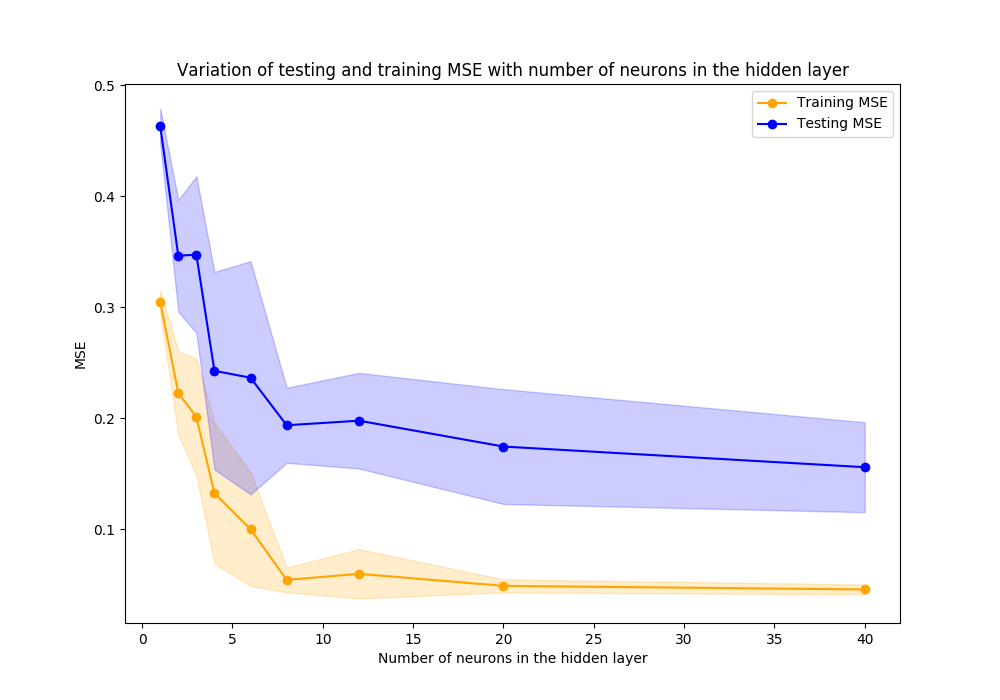
\includegraphics[width=\textwidth]{figures/1_1_c.png}
	\caption{Varying the number of hidden neurons}
	\label{1_1_c}
\end{figure}

\textbf{Discussion}

\begin{itemize}
  \item Best $h_n$ would be $40$ on the Testing Set and $20$ (already) on the
  Training Set (recommend ``Early Stopping'', no significant $\Delta$ after
  $20$).
  \item Different random seed in combination with low $h_n$ can have effects
  either way, under- as well as overfitting tendencies.
  \item Starting with a little underfitting but getting less with growing $h_n$.
\end{itemize}

%%%%%%%%%%%%%%%%%%%%%%%%%% 1.1 d)

  \item \textbf{Variations of MSE during training}
  
Warm up method used and fitting for 1000 iterations with different number of
neurons in a single hidden layer.

\begin{figure}[H]
	\centering
  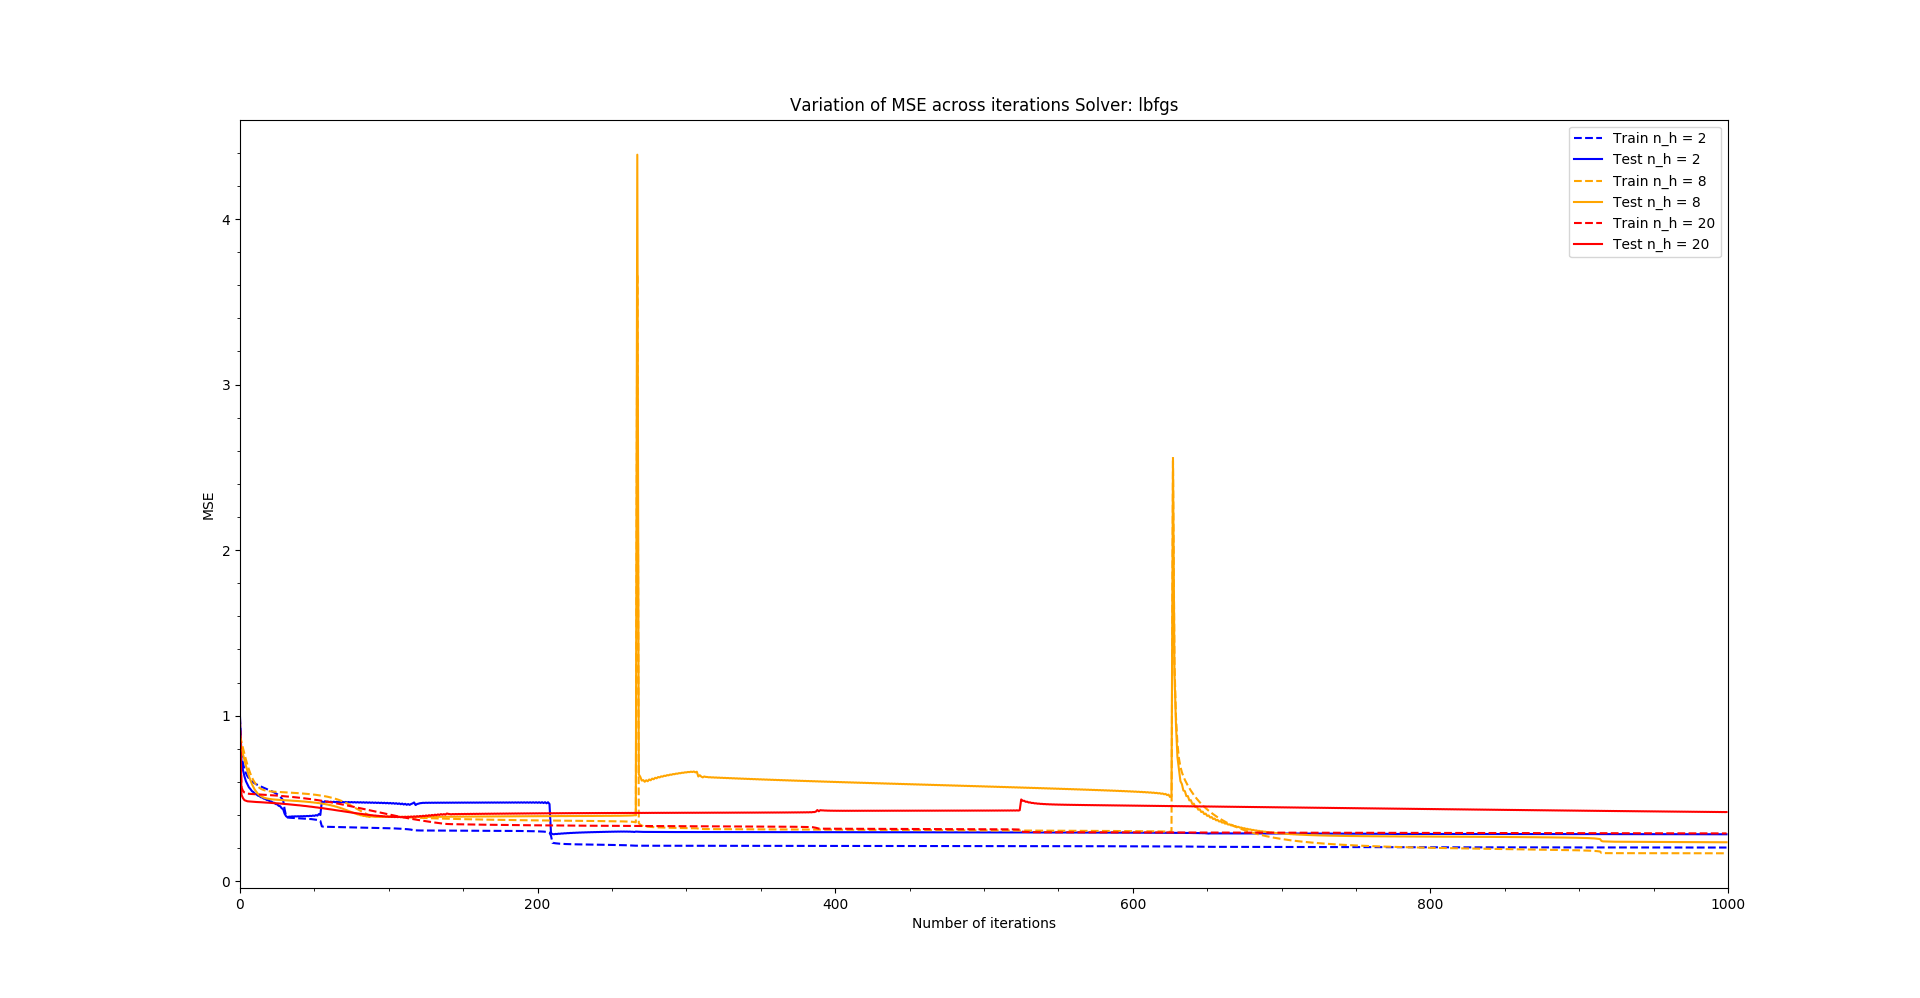
\includegraphics[width=\textwidth]{figures/1_1_d_lbfgs.png}
	\caption{Warm up with up to 1000 iterations using lbfgs solver}
	\label{1_1_d_lbfgs}
\end{figure}

\begin{figure}[H]
	\centering
  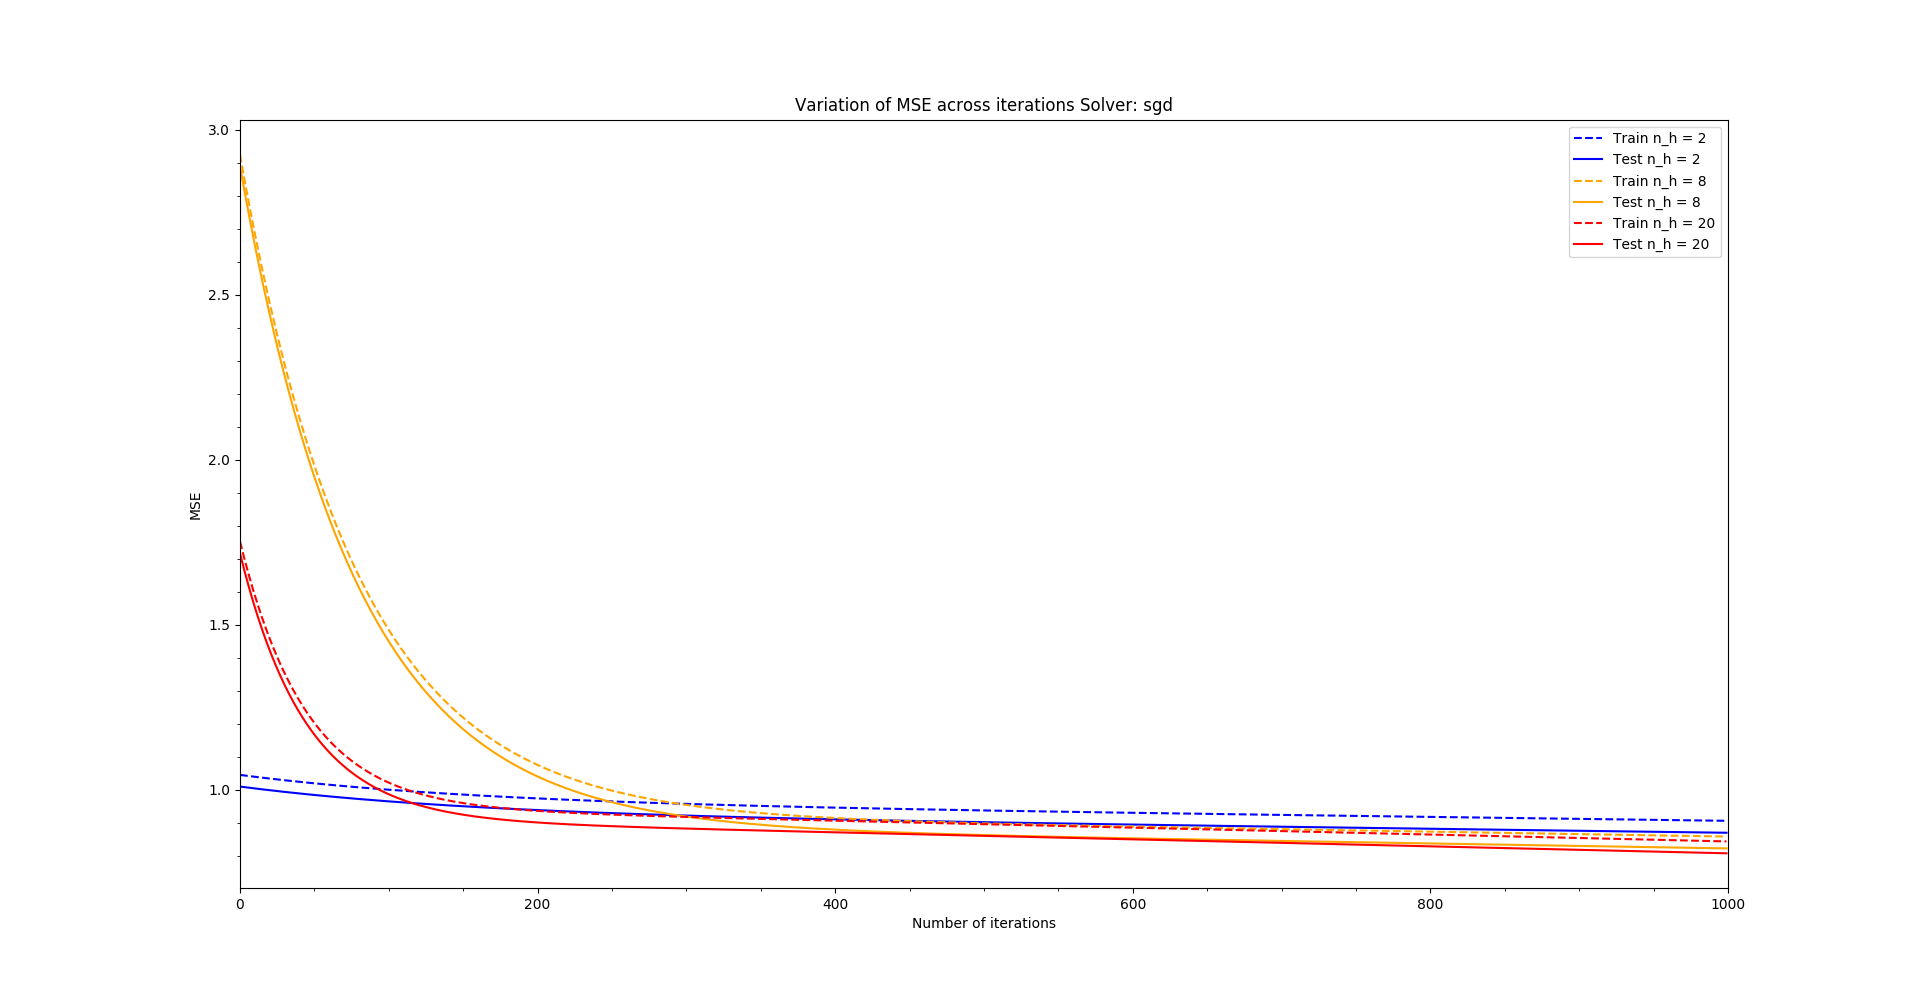
\includegraphics[width=\textwidth]{figures/1_1_d_sgd.png}
	\caption{Warm up with up to 1000 iterations using SGD solver}
	\label{1_1_d_sgd}
\end{figure}

\begin{figure}[H]
	\centering
  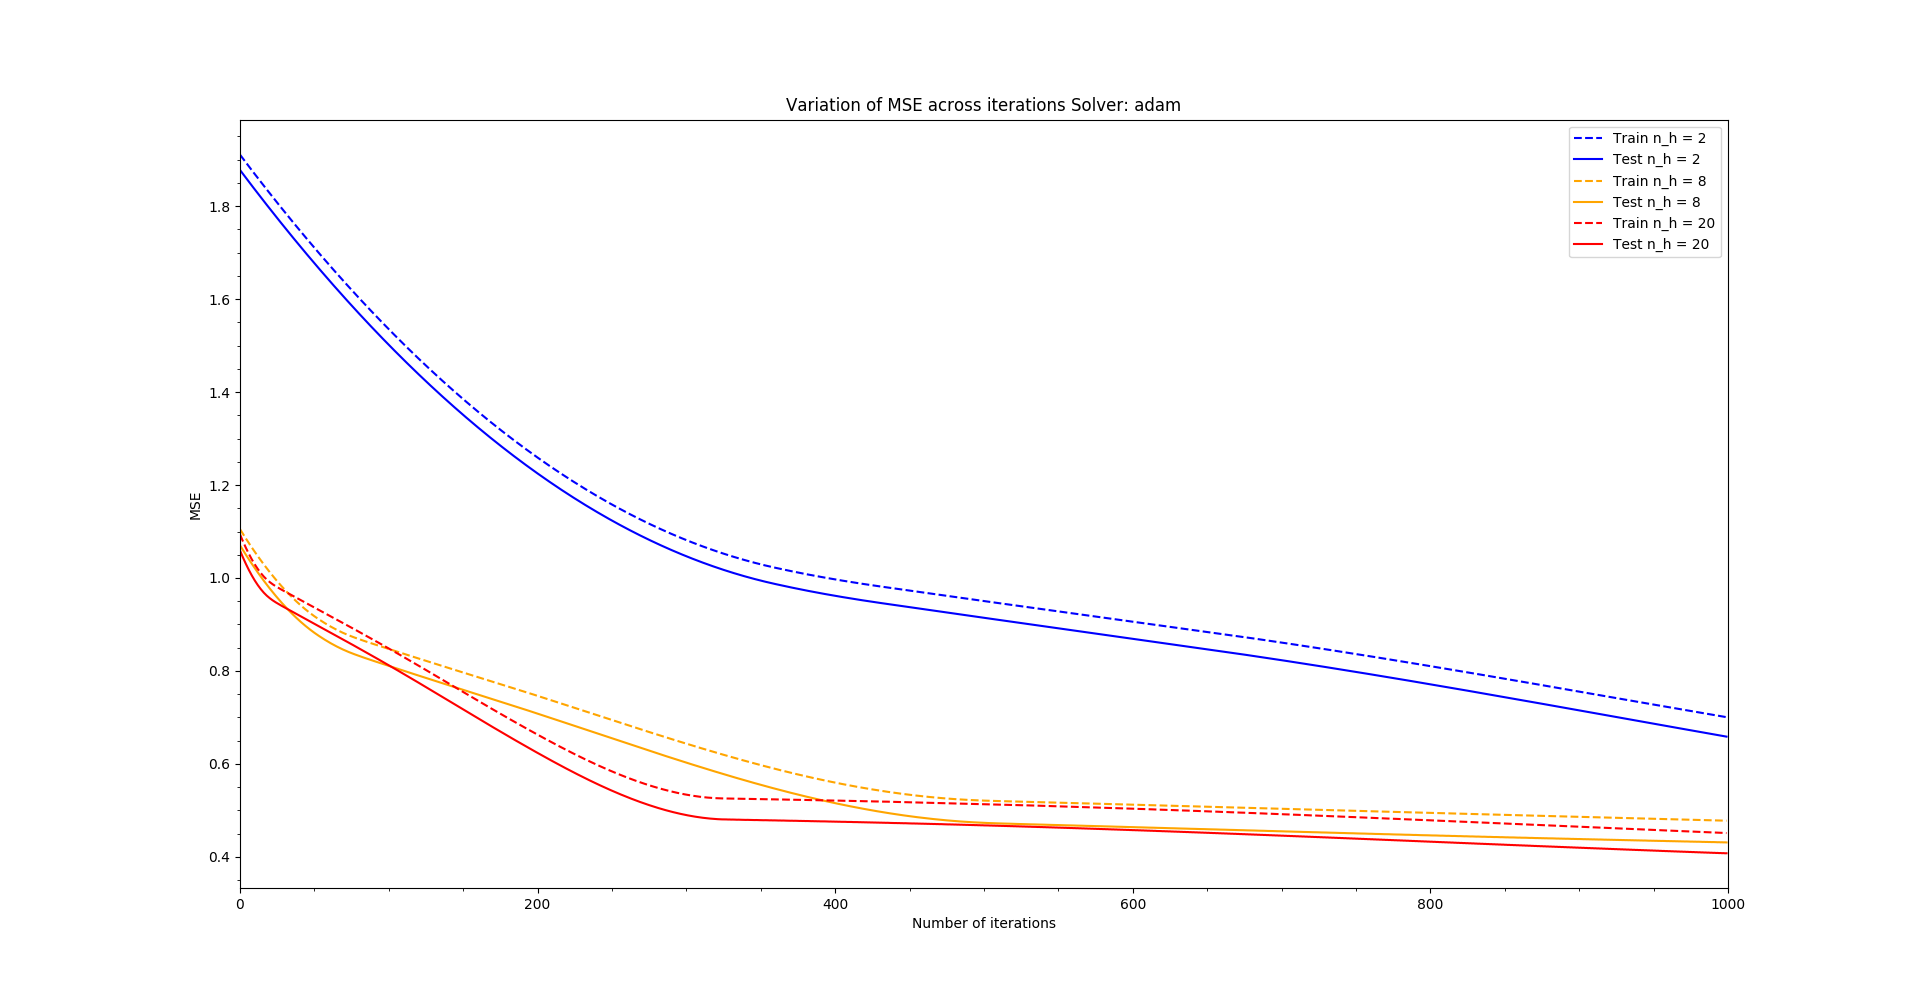
\includegraphics[width=\textwidth]{figures/1_1_d_adam.png}
	\caption{Warm up with up to 1000 iterations using adam solver}
	\label{1_1_d_adam}
\end{figure}

\textbf{Discussion}

\begin{itemize}
  \item Risk of overfitting increases with number of hidden neurons.
  \item Simple SGD would be the best choice for the given dataset (min MSE very
  early with no extreme fitting errors, but slow).
  \item Choosing the correct solver for real-life problems would depend on many
  circumstances
  \begin{itemize}
	  \item Is your analysis time critical (low-latency, Robot, Web-API)? One could
	  reduce complexity and computation time in choosing SGD-like solver (only
	  picking one sample at first, linear runtime). Also number of neurons can be
	  reduced with the risk of underfitting.
	  \item Depending on your input (test data) solvers like adam would perform
	  better on small sets.
	  \item With increasing number of neurons you should use optimized algorithms
	  like adam (fitting risks) or if only few memory is available (robots) you
	  can use lbfgs\autocite{wiki:lbfgs}.
  \end{itemize}
\end{itemize}

\end{enumerate}


\subsection{Regularized Neural Networks}

\begin{enumerate}[a)]
  
%%%%%%%%%%%%%%%%%%%%%%%%%% 1.2 a)
  
  \item \textbf{Weight Decay}
  
Training NN with different values for regularization to combat fitting problems.
  
\begin{figure}[H]
	\centering
  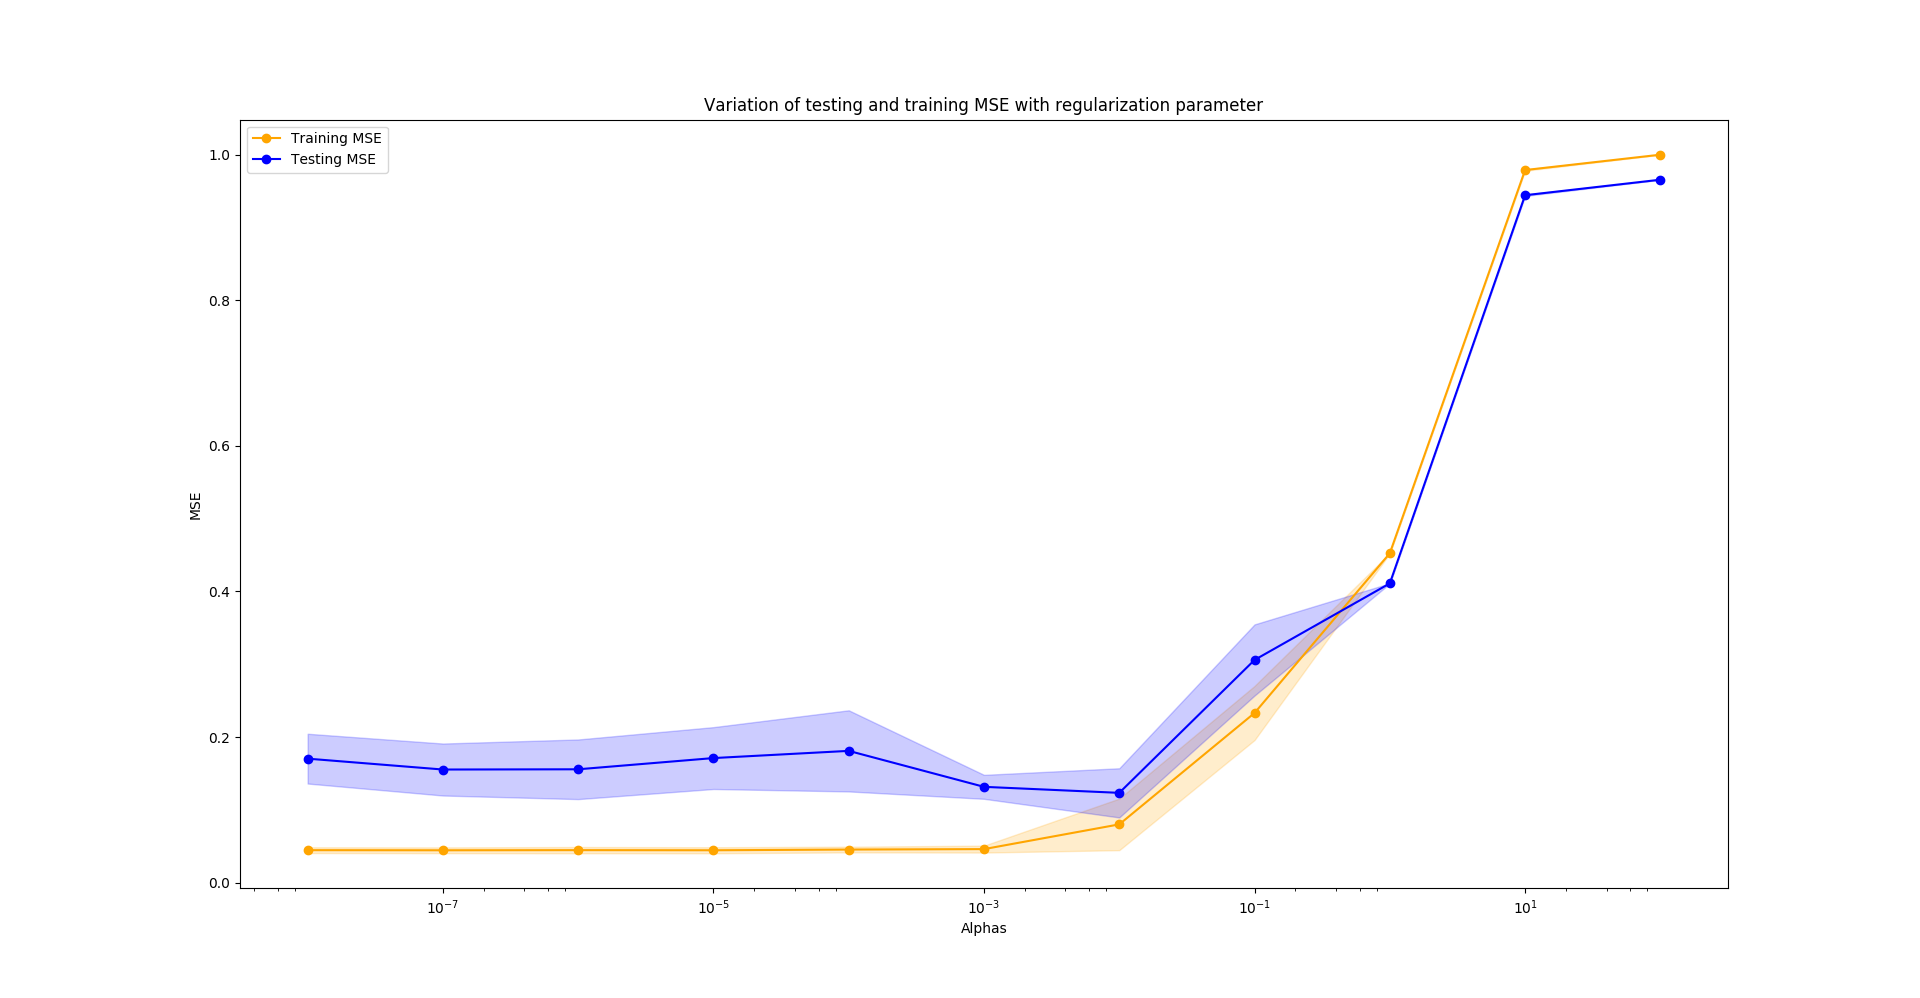
\includegraphics[width=\textwidth]{figures/1_2_a.png}
	\caption{Weight Decay, Training using differen values for regularization}
	\label{1_2_a}
\end{figure}

\textbf{Discussion}

\begin{itemize}
  \item Best value for $\alpha$ on given data would be $10^{-3}$ quite
  independent from seed.
  \item Alpha can help with overfitting by
  constraining the size of wights (lesser
  vurvatures, fix high variance)\autocite{scikit:regularization}. Decreasing
  alpha might also fix high bias and therefore underfitting.
\end{itemize}

%%%%%%%%%%%%%%%%%%%%%%%%%% 1.2 b)
  
  \item \textbf{Early Stopping}

Collecting statistics at which MSE values early stopping would happen when using
part of the training set as validation set. In this case every second sample of
of the training set will be used as validation set.

\begin{figure}[H]
	\centering
  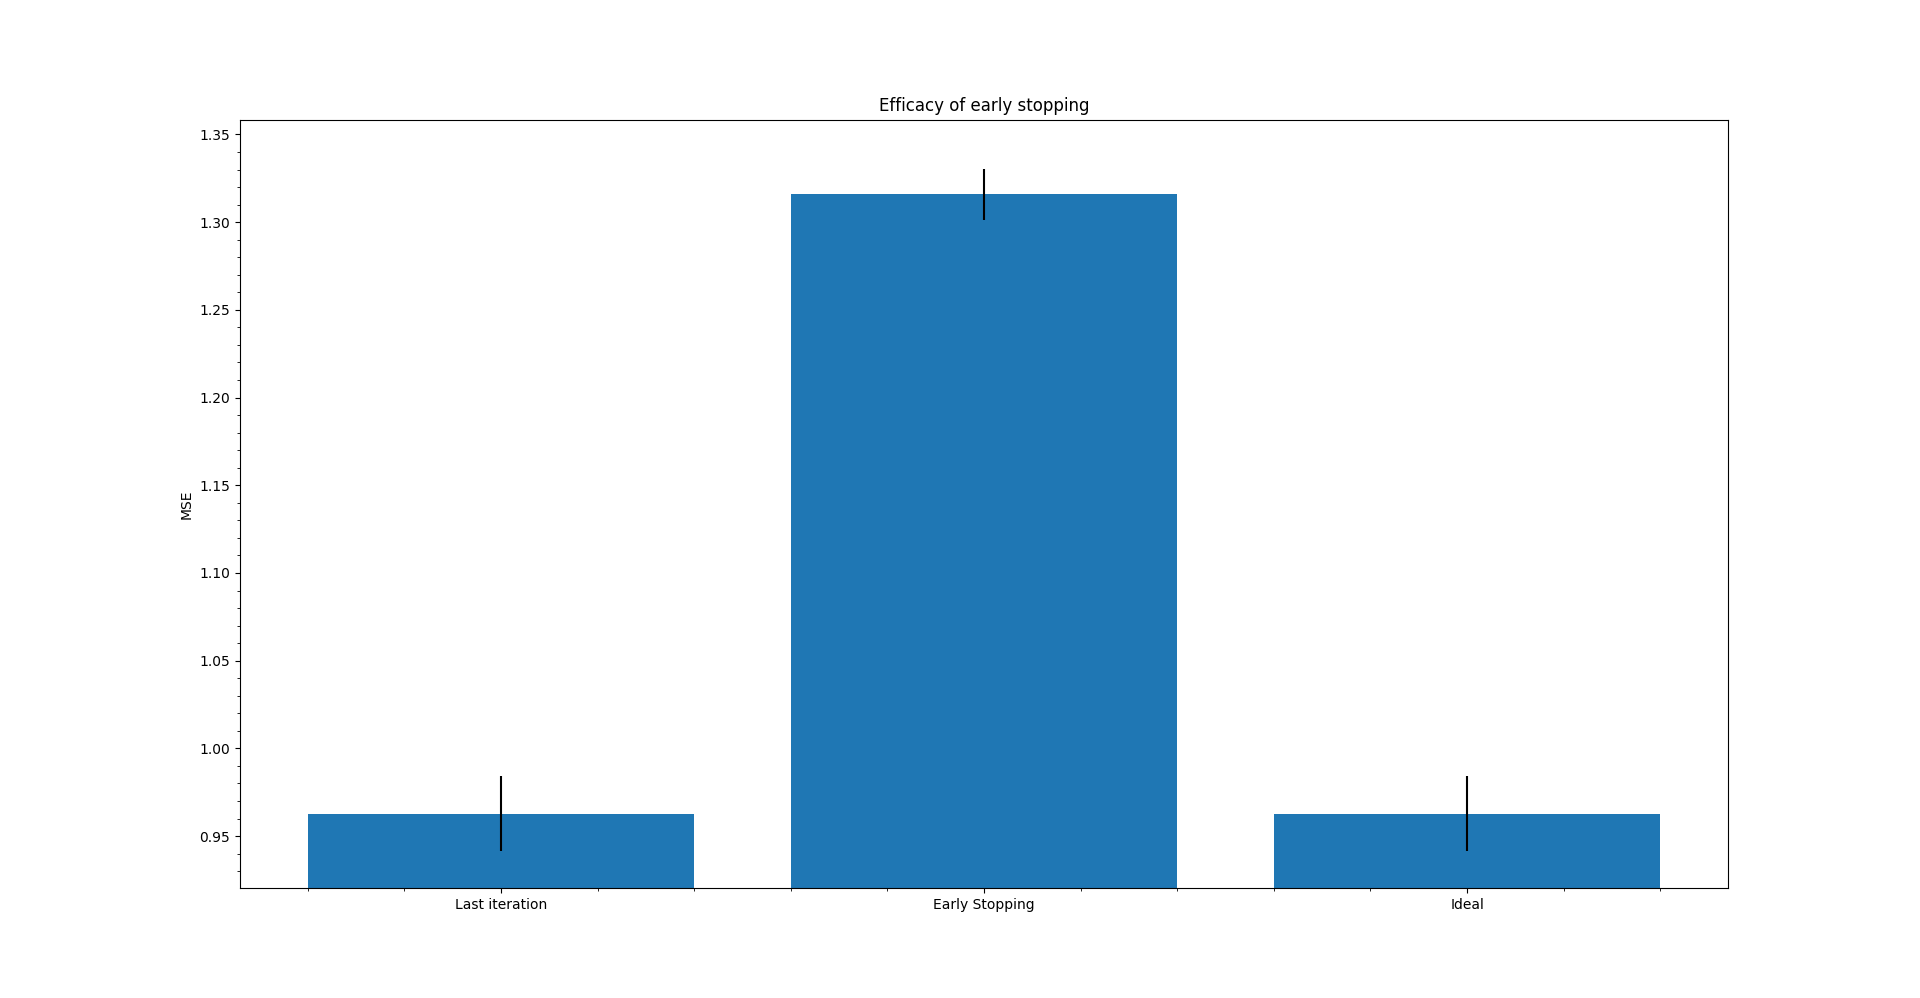
\includegraphics[width=\textwidth]{figures/1_2_b.png}
	\caption{Early stopping MSE Comparison}
	\label{1_2_b}
\end{figure}

\textbf{Discussion}

\begin{itemize}
  \item Either validation set is poorly choosen (every second sample of
  training set) or early stopping would happen at MSE around $1.3$.
  \item In the light of MSE from fittings and evaluation before early stopping
  would improve computation. See comments in discussions before.
\end{itemize}

%%%%%%%%%%%%%%%%%%%%%%%%%% 1.2 c)
  
  \item \textbf{Combining the tricks}
  
\textbf{Decisions}

\begin{itemize}
  \item $n_h = 8$ from Figure \ref{1_1_a_hn_8} and Figure \ref{1_1_c}.
  \item $\textnormal{solver} = SGC$ from Figure \ref{1_1_d_sgd} compared to
  Figure \ref{1_1_d_adam} and Figure \ref{1_1_d_lbfgs}.
  \item Using early stopping parameter for neural network API
  (\texttt{early\_stopping = True}) from Figure \ref{1_2_b}.
  \item $\alpha = 10^{-3}$ derived from Figure \ref{1_2_a}.
  \item min MSE: $0.4787516928151623$ at seed: $4.0$
\end{itemize}

\textbf{Results}

\texttt{Training MSE \\
- min = 0.5278345203427149 \\
- max = 1.5830727895816807 \\
- mean = 0.8633455019924664 \\
- std = 0.3563329403361676\\
Test MSE \\
- min = 0.4787516928151623 \\
- max = 1.5500468662266857 \\
- mean = 0.8232890101751599 \\
- std = 0.36152875307393956\\
}

\textbf{Not ``perfect''} but analysis says this is it.

\end{enumerate}

\section{Face Recognition with Neural Networks}

\begin{figure}[H]
	\centering
  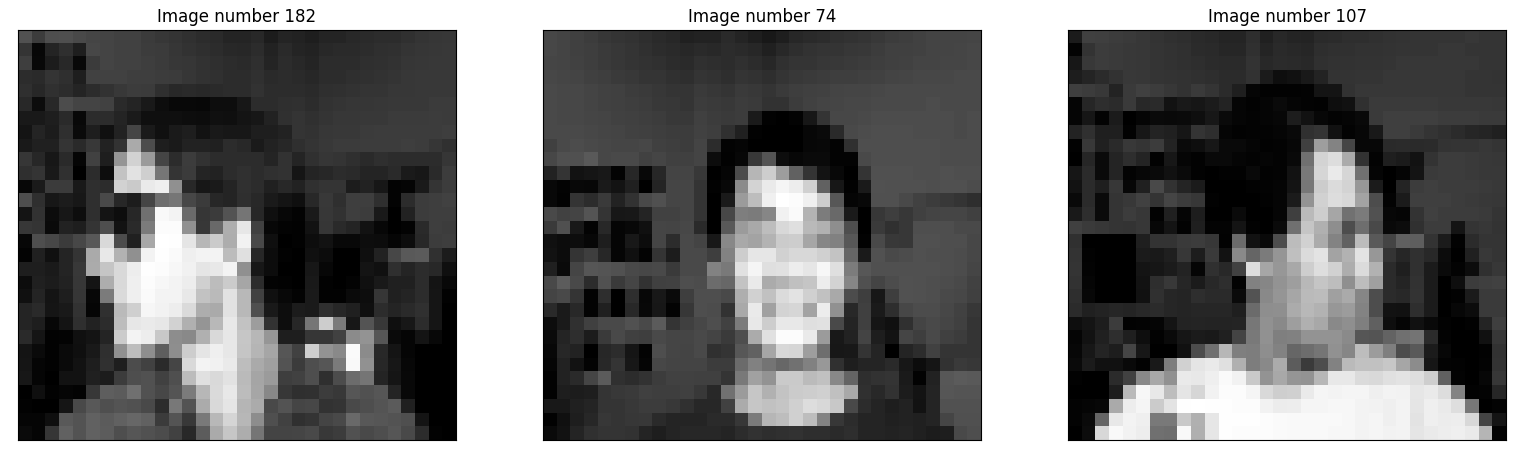
\includegraphics[width=\textwidth]{figures/2_images.png}
	\caption{Example Images}
	\label{2_images}
\end{figure}

\subsection{Pose Recognition}

\textbf{Images}

\textbf{Confusion matrix}

\begin{align*}C =
\begin{pmatrix}
126 & 4 & 5 & 6 \\
3 & 136 & 0 & 2 \\
0 & 1 & 133 & 4 \\
11 & 5 & 2 & 126
\end{pmatrix}
\end{align*}

\begin{center}
\begin{tabular}{| r | c | c | c | c | }
\hline
& \rotatebox{90}{straight} & \rotatebox{90}{left} & \rotatebox{90}{right} &
\rotatebox{90}{up} \\
\hline
straight & \textcolor{green}{\textbf{126}} & \textcolor{red}{\textbf{4}} &
\textcolor{red}{\textbf{5}} & \textcolor{red}{\textbf{6}} \\
\hline 
left & \textcolor{red}{\textbf{3}} & \textcolor{green}{\textbf{136}} & 0 &
\textcolor{red}{\textbf{2}} \\ 
\hline 
right & 0 & \textcolor{red}{\textbf{1}} & \textcolor{green}{\textbf{133}} &
\textcolor{red}{\textbf{4}} \\
\hline 
up & \textcolor{red}{\textbf{11}} & \textcolor{red}{\textbf{5}} &
\textcolor{red}{\textbf{2}} & \textcolor{green}{\textbf{126}} \\ \hline
\end{tabular}
\end{center}

\textbf{Discussion}

\begin{figure}[H]
	\centering
  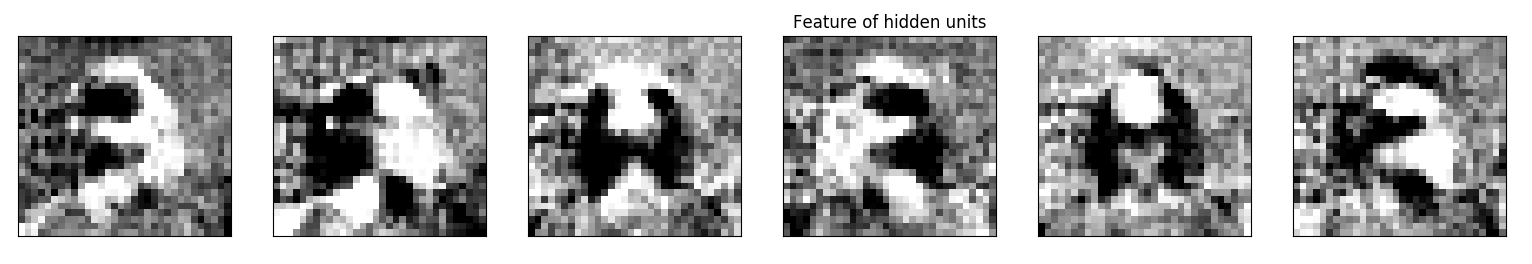
\includegraphics[width=\textwidth]{figures/2_1_coeff.png}
	\caption{Weight in hidden layers}
	\label{2_1_coeff}
\end{figure}


\begin{itemize}
  \item There seems to be less confusion on left and right than on up
  (especially in combination with straight).
  \item sunglasses, hair, nose, eyes seems to get more weight
\end{itemize}

\subsection{Face Recognition}

\printbibliography

\end{document}